\documentclass[a4paper,10pt]{article}
\usepackage[utf8]{inputenc}

\title{Notes about theory of merge}
\author{Guillaume Bertholon}

\usepackage{listings-rust}
\lstset{
  language=Rust,
  breaklines=true,
  extendedchars=true,
  captionpos=b,
  style=boxed
}

\usepackage{tikz}
\usetikzlibrary{calc}
\usetikzlibrary{positioning}
\tikzstyle{varnode} = [draw, circle, text height=1.5ex, text depth=.25ex, align=center]
\tikzstyle{modnode} = [draw, rectangle]

\begin{document}

\maketitle

How can we compose simulataneous changes?

\section{A key principle: mandatory disambiguation}
\paragraph{Commits \& modifications}
In this section, I will have a very generic notion of commits. A commit is a set of modifications of the semantic of a program. A single modification
can have an impact on several program states and several program variables.
An example of a modification is the change of an expression in an assignment (\lstinline{x = expr}). This modification does not only touch the program variable \lstinline{x} but also each expression that depend the new value in the rest of the program.
\begin{lstlisting}[caption=Modification of $x$]
let mut x = 0; // changed
let y = x + 1; // touched (x is changed)
let z = y + 1; // touched (y is touched)
x = 45;        // untouched
let w = x - 3; // untouched (x have been reassigned)
\end{lstlisting}
Inside a commit we consider that all the modifications are compatible with each
other as their author have thought of their potential interactions.
With this idea of thoughtful interactions, we can consider that sequential commits can always be (virtually) squashed into a single commit before merging.

\paragraph{Concurrent commits}
Concurrent commits are commits that all transform the same initial program. Their authors were not aware of the modifications contained in other commits. Nonetheless, we want to be able to merge the modifications contained in all of them inside a single commit from the common source. A merged version is not always uniquely well-defined because concurrent modifications can (and will often) touch the same program states or variables and therefore collide. That's why there can be several merged versions of the same set of concurrent commits.

Sometimes however they will never collide and a canonical merge commit will naturally exist. This is the case for instance if two incompatible branches are modified by concurrent commits.
\begin{lstlisting}[caption=Merged version of two compatible concurrent commits modifying $x$]
let x;
if (c) {
    x = 1; // changed in first concurrent commit
} else {
    x = 2; // changed in second concurrent commit
}
let y = x + 1; // touched but unambiguous
\end{lstlisting}

\paragraph{A generic definition of a valid merge} A merge is valid if for any state of the program, there is a single unambiguous trace after applying all the modifications of the concurrent commits. There should be no automatic choice in favor of any of the commits. This means that if two commits touched the same state of the program or the same variable at the same time, the merge will be considered not valid. We call a point in a trace where the semantic is ambiguous a collision.
Note that I consider that this includes a case where commit $A$ modifies a variable $x$ and then commit $B$ changes the value of $y$ to the new value of $x$.

\noindent
\begin{minipage}{.32\textwidth}
\begin{lstlisting}
// Commit A
let x = 2;
let y = 3;
\end{lstlisting}
\end{minipage}\hfill
\begin{minipage}{.32\textwidth}
\begin{lstlisting}
// Original
let x = 1;
let y = 3;
\end{lstlisting}
\end{minipage}\hfill
\begin{minipage}{.32\textwidth}
\begin{lstlisting}
// Commit B
let x = 1;
let y = x; // !!!
\end{lstlisting}
\end{minipage}
\vspace{-.4cm}
\begin{lstlisting}[caption=Colliding changes by using a variable modified by someone else]
\end{lstlisting}

To keep track of potential collisions we can create a graph of origins that is updated between each program state. This graph has a node for each variable plus one node for each modification (labelled by the commit). Two nodes are linked by an edge if the value of a variable comes from the value of another variable or comes directly from a modification.

If at a given point of a program, a node of the origin graph is transitively linked to modifications of different concurrent commits, then there is a collision at this point.

\begin{figure}[ht]
\centering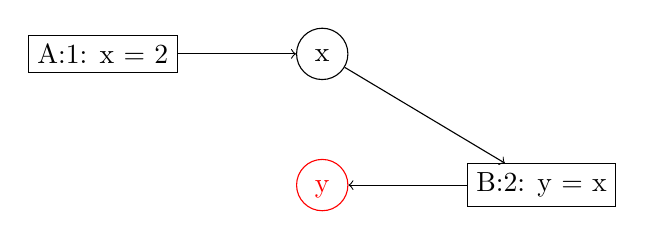
\begin{tikzpicture}
  \node[varnode] (x) {x};
  \node[varnode, below=1cm of x, red] (y) {y};

  \node[modnode, left=1.5cm of x] (x_A) {A:1: x = 2};
  \draw[->] (x_A) -- (x);

  \node[modnode, right=1.5cm of y] (y_B) {B:2: y = x};
  \draw[->] (x) -- (y_B);
  \draw[->] (y_B) -- (y);
\end{tikzpicture}
\caption{Illustration of the origin graph of the previous program. There is a collision for $y$ because it is both linked to a modification in $A$ and a modification in $B$.}
\end{figure}

\begin{figure}[ht]
\begin{minipage}{.5\textwidth}
\begin{lstlisting}
let a = 0; // Modified by A
let b = 1; // Modified by B
let c = a + b; // Collision
\end{lstlisting}
\end{minipage}\hfill
\begin{minipage}{.45\textwidth}
\centering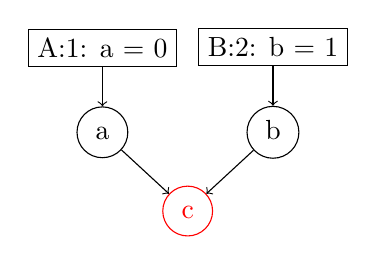
\begin{tikzpicture}
  \node[varnode] (a) {a};
  \node[varnode, right=1.5cm of a] (b) {b};
  \node[varnode, red] (c) at ($(a)!0.5!(b)+(0,-1)$) {c};

  \node[modnode, above=0.5cm of a] (A_a) {A:1: a = 0};
  \node[modnode, above=0.5cm of b] (B_b) {B:2: b = 1};

  \draw[->] (A_a) -- (a);
  \draw[->] (B_b) -- (b);
  \draw[->] (a) -- (c);
  \draw[->] (b) -- (c);
\end{tikzpicture}
\end{minipage}
\caption{Collision created after modification of two independant variables}
\end{figure}

\paragraph{Origin graph and control flow} If the value of a variable is used for defining control flow, it will gain create a dependancy on all the variables inside the branches.

\begin{figure}[ht]
\begin{minipage}{.5\textwidth}
\begin{lstlisting}
let a = 2;
let b = 5;
let c = a;
while (c < b) {
    c += 1;
}
\end{lstlisting}
\end{minipage}\hfill
\begin{minipage}{.45\textwidth}
\centering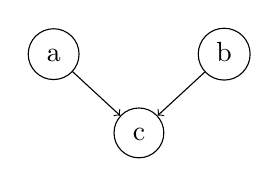
\begin{tikzpicture}
  \node[varnode] (a) {a};
  \node[varnode, right=1.5cm of a] (b) {b};
  \node[varnode] (c) at ($(a)!0.5!(b)+(0,-1)$) {c};

  \draw[->] (a) -- (c);
  \draw[->] (b) -- (c);
\end{tikzpicture}
\end{minipage}
\caption{Origin graph at the end of a program containing a while-loop. Note that $c$ keeps its dependancy on $a$ as it used its previous value inside the loop.}
\end{figure}

However incompatible branches can be treated independantly and do not generate conflicts by themselves.
\begin{figure}[ht]
\begin{minipage}{.5\textwidth}
\begin{lstlisting}
let b = 2; // Modified by B
let x;
if (c) {
    x = 1; // Modified by A
} else {
    x = b; // Touched by B
}
let y = x - 1; // OK
let z = y + b; // Conflict
\end{lstlisting}
\end{minipage}\hfill
\begin{minipage}{.45\textwidth}
\centering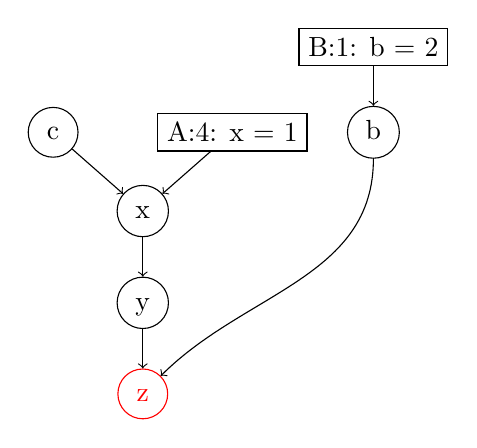
\begin{tikzpicture}
  \node[varnode] (b) {b};
  \node[modnode, above=0.5cm of b] (B_b) {B:1: b = 2};
  \node[modnode, left=0.5cm of b] (A_x) {A:4: x = 1};
  \node[varnode, left=1cm of A_x] (c) {c};
  \node[varnode] (x) at ($(c)!0.5!(A_x)+(0,-1)$) {x};
  \node[varnode, below=0.5cm of x] (y) {y};
  \node[varnode, below=0.5cm of y, red] (z) {z};


  \draw[->] (B_b) -- (b);
  \draw[->] (c) -- (x);
  \draw[->] (A_x) -- (x);
  \draw[->] (x) -- (y);
  \draw[->] (y) -- (z);
  \draw[->] (b) to[out=-90, in=45] (z);
\end{tikzpicture}
\end{minipage}
\caption{Origin graph at the end of a program after taking the then branch, showing that there is no collision on $x$ but still one on $z$.}
\end{figure}

This might become a problem if care is not taken in origin graph checks, because each branch combination might need to be examined.

\paragraph{Solving collisions by overriding}
In order to be able to solve collisions, I extend the definition of a merge with a set of modification overrides in addition to the set of concurrent commits.
A modification in the override set, take precedence over any modification in any of the merged commits. Moreover we can consider that these overrides are done knowing what is inside all the concurrent commits.

In the origin graph, a variable that takes a value defined in by an override modification will loose all incoming arrows as its value is now disambiguated for the current state, taking all further implications into account.

Having a single overriden ancestor can be not enough for marking a conflict as solved though.

\begin{figure}[ht]
\begin{minipage}{.5\textwidth}
\begin{lstlisting}
let a = 0; // modified by A
let b = 1; // modified by B
let o = a + b; // overriden
let c = a + o;
let d = c + b; // Collision!
\end{lstlisting}
\end{minipage}\hfill
\begin{minipage}{.45\textwidth}
\centering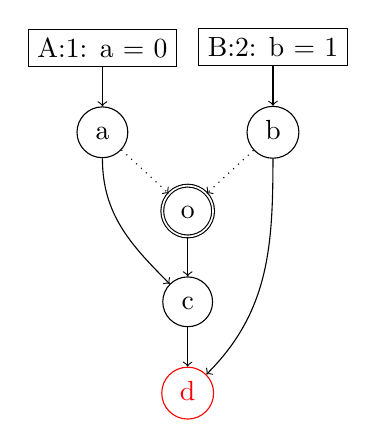
\begin{tikzpicture}
  \node[varnode] (a) {a};
  \node[varnode, right=1.5cm of a] (b) {b};
  \node[varnode, double] (o) at ($(a)!0.5!(b)+(0,-1)$) {o};
  \node[varnode, below=0.5cm of o] (c) {c};
  \node[varnode, below=0.5cm of c, red] (d) {d};

  \node[modnode, above=0.5cm of a] (A_a) {A:1: a = 0};
  \node[modnode, above=0.5cm of b] (B_b) {B:2: b = 1};

  \draw[->] (A_a) -- (a);
  \draw[->] (B_b) -- (b);
  \draw[->, dotted] (a) -- (o);
  \draw[->, dotted] (b) -- (o);
  \draw[->] (o) -- (c);
  \draw[->] (c) -- (d);
  \draw[->] (a) to[out=-90,in=135] (c);
  \draw[->] (b) to[out=-90,in=45] (d);
\end{tikzpicture}
\end{minipage}
\caption{Origin graph for a merge with an overriding that solves one conflict line 3 but is insufficient to also solve the conflict line 5. Deleted edges are dotted, variables overriden have a double border.}
\end{figure}

A override can arbitrarily alter a modification, or even touch something that was not modified to restore the intent of both modifications. In the example above, $o$ might have been untouched neither by $A$ or by $B$ or be touch by one of the commits or by both, it doesn't matter. That's why an override is also a way to state the behaviour of the program when the changes are on the same state.

Usually there can be several way to solve the same conflict, but some are more ``powerful'' than others. A variable assigned to an overriden expression should be considered as a variable with a restored semantic with respect to all the modifications.

\begin{figure}[ht]
\begin{minipage}{.5\textwidth}
\begin{lstlisting}
let a = 0; // modified by A
let b = 1; // overriden
let o = a + b;
let c = a + o;
let d = c + b;
\end{lstlisting}
\end{minipage}\hfill
\begin{minipage}{.45\textwidth}
\centering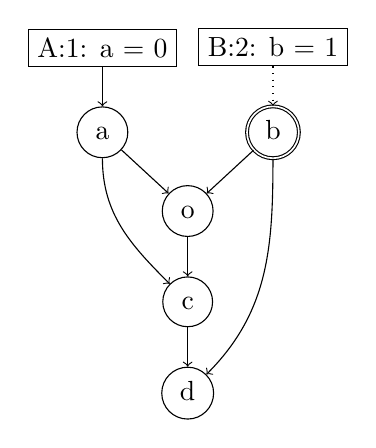
\begin{tikzpicture}
  \node[varnode] (a) {a};
  \node[varnode, right=1.5cm of a, double] (b) {b};
  \node[varnode] (o) at ($(a)!0.5!(b)+(0,-1)$) {o};
  \node[varnode, below=0.5cm of o] (c) {c};
  \node[varnode, below=0.5cm of c] (d) {d};

  \node[modnode, above=0.5cm of a] (A_a) {A:1: a = 0};
  \node[modnode, above=0.5cm of b] (B_b) {B:2: b = 1};

  \draw[->] (A_a) -- (a);
  \draw[->, dotted] (B_b) -- (b);
  \draw[->] (a) -- (o);
  \draw[->] (b) -- (o);
  \draw[->] (o) -- (c);
  \draw[->] (c) -- (d);
  \draw[->] (a) to[out=-90,in=135] (c);
  \draw[->] (b) to[out=-90,in=45] (d);
\end{tikzpicture}
\end{minipage}
\caption{Origin graph for the same example as before except that now line 2 is
overriden marking that $b$ has a preserved semantic. Therefore, line 5 is not showing a conflict anymore.}
\end{figure}

\section{Modification of expressions only}
This idea works very well for commits that only consist of modifications of expressions and preserve the whole program structure (but maybe not the control flow).

\end{document}
